\chapter{The Daya Bay Experiment}

\section{The Daya Bay Site}
To measure $\theta_{13}$, an experimental site with reactors of high thermal power to supply large antineutrino flux and with mountains nearby to serve as cosmic ray shielding is required. Daya Bay is an appropriate site meeting the requirements.

The Daya Bay reactor complex is located on the southeast coast of China, 55 km northeast of Hong Kong. The reactor complex is composed of 3 nuclear power plants, namely the Daya Bay (DYB) nuclear power plant, the Ling Ao (LA) nuclear power plant, and the Ling Ao-II (LA II) nuclear power plant. Each nuclear power plant is equipped with a pair of functionally identical pressurized water reactors (PWR) separated by 90 m. Each reactor core supplies 2.9 GW thermal power. The last core going online started commercial operation in August, 2011. The Ling Ao nuclear power plant is \textasciitilde 1100 m from the Daya Bay nuclear power plant, and the Ling Ao-II is \textasciitilde 500 m from the Ling Ao.

The Daya Bay experimental facility is composed of 3 underground experimental halls, a surface assembly building, a liquid scintillator (LS) hall, and a water hall (EH4). The underground halls are connected by horizontal tunnels. The 3 experimental halls are where the antineutrino detectors and the muon detectors are installed. The experimental hall closest to the Daya Bay/Ling Ao nuclear power plant is called the Daya Bay/Ling Ao near site, or experimental hall 1/2 (EH1/EH2). The experimental hall farthest from all the reactor cores is called the Far site, or experimental hall 3 (EH3). The near sites are designed to hold two antineutrino detectors (ADs) each while the far site is designed to hold four ADs. The surface assembly building is the place where experimenters assemble the ADs, do the dry run tests, and other detector related work before transporting the equipment underground. The LS hall is where Daya Bay's liquid scintillator and Gd-doped liquid scintillator are produced, and is where the ADs are filled. The water hall is where the ultra-pure water system is placed which supplies ultra-pure water to the 3 water pools in EH1, EH2, and EH3. Figure~\ref{fig:dybsite} shows the experimental facility and the 6 reactor cores. The distances from the centroid of the reactor pairs to the sites are shown in Table~\ref{tab:sitecoredist}. The Global Positioning System (GPS) and modern theodolites are utilized to survey all distances. The uncertainty of the baselines from the geometric center of the reactor cores to the AD centers was determined to be about 28 mm~\cite{dayabay2012_1}.

\begin{figure}
	\centering
	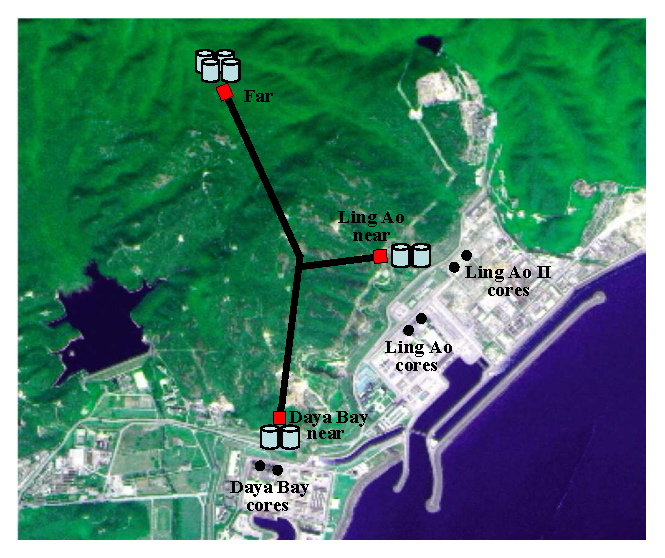
\includegraphics[width=0.45\textwidth]{figures/chap3/dayabay_site.eps}
	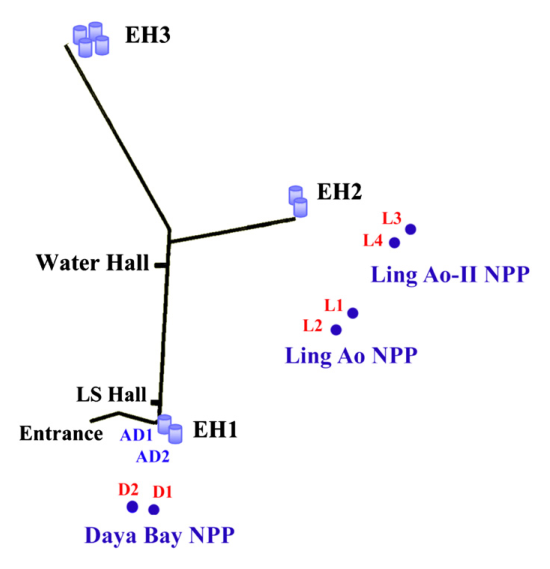
\includegraphics[width=0.35\textwidth]{figures/chap3/dayabay_site_illustration.eps}
	\caption{The Daya Bay site.}
	\label{fig:dybsite}
\end{figure}

\begin{table}
	\centering
	\begin{tabular}{|c|c|c|c|}
	\hline
	& DYB & LA & FAR \\
	\hline
	DYB cores & 363 & 1347 & 1985 \\
	\hline
	LA cores & 857 & 481 & 1618 \\
	\hline
	LA II cores & 1307 & 526 & 1613 \\
	\hline
	\end{tabular}
	\caption{Distances from the centroids of each reactor pair to the sites.}
	\label{tab:sitecoredist}
\end{table}
The overburden in equivalent meters of water (m.w.e.), simulated muon rate and average muon energy are listed in Table~\ref{table:muon_rate}.
\begin{table}
	\centering
	\begin{tabular}{cccc}
		\toprule
		& Overburden (m.w.e.) & $R_\mu$ (Hz/m$^2$) & $\left\langle E_\mu \right\rangle$ (GeV) \\
		\midrule
		EH1 & 250 & 1.27 & 57 \\
		EH2 & 265 & 0.95 & 58 \\
		EH3 & 860 & 0.056 & 137 \\
		\bottomrule
	\end{tabular}
	\caption{Vertical overburden, muon rate $R_\mu$, and average muon energy $\left\langle E_\mu \right\rangle$ of the three EHs.}
	\label{table:muon_rate}
\end{table}


\section{The Antineutrino Detector}

The antineutrino detectors (ADs) are the main detectors used for detecting neutrinos via the inverse beta decay reaction. Figure~\ref{fig:CSAD} shows the cross sectional view of the Daya Bay AD. The AD is separated into 3 different zones by 3 coaxial cylindrical vessels. From outside to inside, they are the stainless steel vessel (SSV), the outer acrylic vessel (OAV) and the inner acrylic vessel (IAV). The SSV is a 5-meter high cylinder with a 5-meter diameter. The OAV is a 4-meter high cylinder with a 4-meter diameter while the IAV is a 3-meter high cylinder with a 3-meter diameter. Inside the IAV is the neutrino target filled with 20 tons liquid scintillator (LS) doped with gadolinium (Gd). The concentration of Gd in the LS is $0.1\%$ by weight. Twenty tons of unloaded liquid scintillator is filled between the IAV and the OAV which serves as the gamma catcher. The outermost region between the IAV and the SSV is filled with 37 t of mineral oil and is call the buffer layer.
\begin{figure}
	\centering
	\includegraphics[width=0.7\textwidth]{figures/chap3/AD_cross_section.eps}
	\caption{Cross sectional view of the Daya Bay antineutrino detector.}
	\label{fig:CSAD}
\end{figure}
The gamma catcher is to capture photons leaving the target area, which relieves Daya Bay's data analysis of a fiducial volume cut which could introduce a large uncertainty. The buffer layer is to shield the target area from radioactivity in the PMTs or the SSV.
Each antineutrino detector is equipped with 192 8-inch Hamamatsu R5912 PMTs~\cite{Hamamatsu} mounted on 8 ladders along the circumference of the SSV and within the mineral oil region. The PMTs are arranged in 24 columns and 8 rings. Two specular reflectors are installed above and below the LS volume to increase the photo-coverage from 6\% to 12\%.

Three Automated Calibration Units (ACU-A, ACU-B, and ACU-C) are mounted on the top of the SSV of each AD as shown in Figure~\ref{fig:dayabay_detectors}. Each ACU contains three sources which are listed in Table~\ref{table:ACU_sources}. The sources can be deployed to better than 0.5 cm along a vertical line down to the bottom of the acrylic vessels.
\begin{figure}
	\centering
	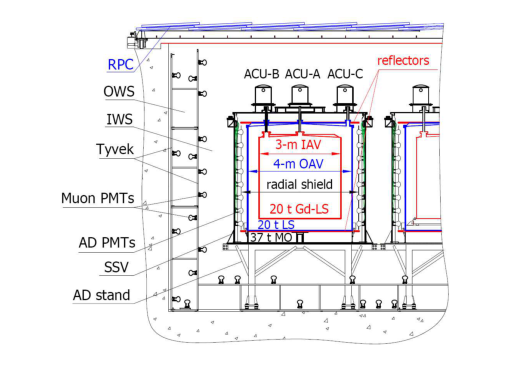
\includegraphics[width=0.7\textwidth]{figures/chap3/dayabay_detectors.eps}
	\caption{Schematic diagram of the Daya Bay detectors.}
	\label{fig:dayabay_detectors}
\end{figure}
\begin{table}
	\centering
	\begin{tabular}{ccc}
		\toprule
		source & particle & frequency (Hz) \\
		\midrule
		$^{68}$Ge & $\beta^+$ & 15 \\
		\hline
		$^{241}$Am-$^{13}$C & n & 0.5 \\
		and $^{60}$Co & $\gamma$ & 100 \\
		\hline
		LED diffuser ball & light & 500 \\
		\bottomrule	
	\end{tabular}
	\caption{Sources in an ACU and their properties.}
	\label{table:ACU_sources}
\end{table}

\subsection{The Liquid Scintillator}
Liquid scintillators (LS) usually serve as a neutrino target, and have advantages such as being cheap, easy to scale up, and easy to dope with elements. Liquid scintillators are commonly composed of two parts, the solvent and the phosphors. Aromatic organics are proven to be good solvents for LS. The electrons in the solvent molecules capture the energy of incident particles. However the solvent molecules usually have little tendency to emit light. Phosphors are added to convert the absorbed energy into light. Two classes of phosphors are usually involved in the LS, the primary scintillators and the wavelength shifters. When the solvent molecules with absorbed energy meet primary scintillator molecules, the energy gets transferred to the scintillator and light is emitted. However this light is usually in the short wavelength region, where PMTs usually have low quantum efficiency. Therefore the wavelength shifters are added to absorb and re-emit the light in the longer wavelength, usually visible light region.

Daya Bay uses linear alkylbenzene (LAB), which was also adopted by the SNO experiment, as the LS solvent~\cite{Beriguete2014}. LAB is known to have good optical transparency, in the order of 10 m, high light yield, low radioactive impurities, and high flash point for safe operation. LAB's chemical composition is basically a straight alkyl chain of 10-13 carbons attached to a benzene ring (Figure~\ref{fig:LAB}). The LS also contains 3 g/L PPO and 15 mg/L Bis-MSB as the primary scintillator and the wavelength shifter, respectively (Figure~\ref{fig:PPO} and Figure~\ref{fig:Bis-MSB}).
\begin{figure}
	\centering
	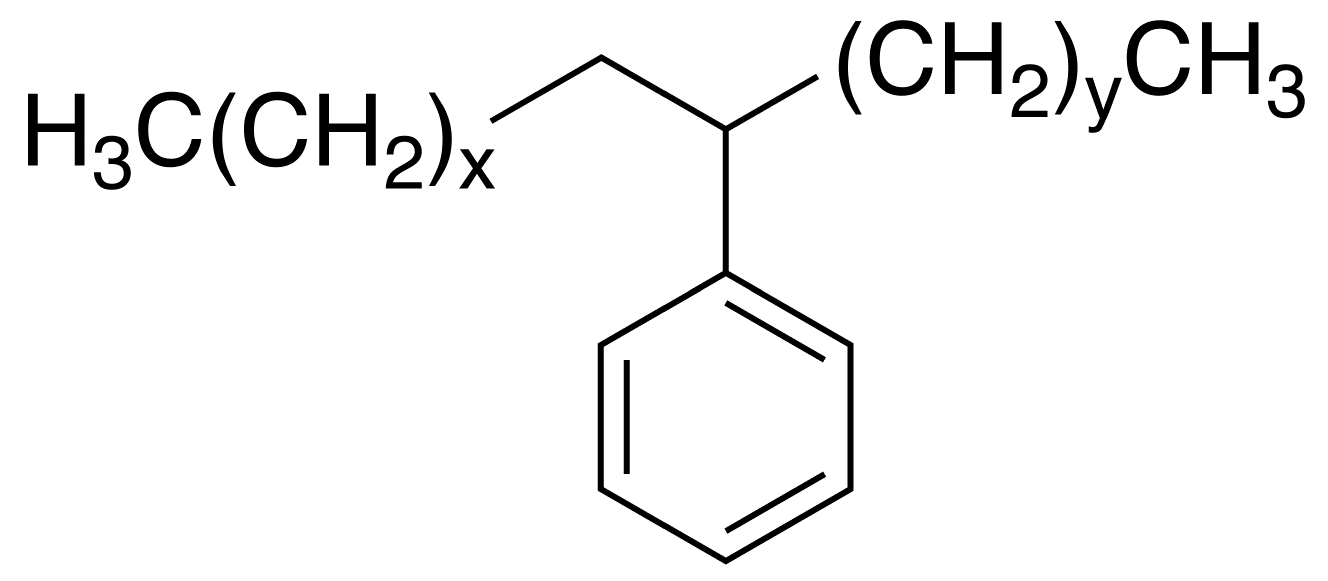
\includegraphics[width=.5\textwidth]{figures/chap3/LAB.png}
	\caption{The Daya Bay liquid scintillator solvent, linear alkylbenzene (LAB).}
	\label{fig:LAB}
\end{figure}
\begin{figure}
	\centering
  \subfloat[Primary scintillator PPO]{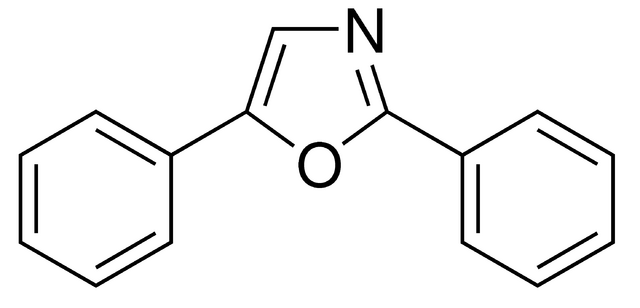
\includegraphics[height=.15\textheight]{figures/chap3/PPO.png}\label{fig:PPO}}
  \qquad
	\subfloat[Wavelength shifter Bis-MSB]{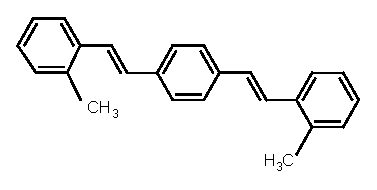
\includegraphics[height=.15\textheight]{figures/chap3/Bis-MSB.eps}\label{fig:Bis-MSB}}
	\caption{The primary scintillator and the wavelength shifter in Daya Bay's LS.}
\end{figure}

Thermalized neutrons in the scintillator can be captured on hydrogen with a mean capture time of $\sim$200 $\mu$s and decay $\gamma$'s of 2.2 MeV. The doping of gadolinium causes neutron capture on Gd with a mean capture time of $\sim$30 $\mu$s and decay $\gamma$'s of 8 MeV. The shorter capture time greatly reduces the rate of accidental coincidence, and the 8 MeV energy is way above the natural radioactivity backgrounds. Besides, the neutron capture cross section on gadolinium is 49,000 barn, more than $10^5$ times larger than the capture cross section on hydrogen ($\sim$0.3 barn). As a consequence, Daya Bay's target LS is doped with $0.1\%$ Gd.

It is seen from Figure~\ref{fig:PPO} that other than carbon and hydrogen, Daya Bay's scintillator contains other elements. Table~\ref{table:LS_composition} and Table~\ref{table:GdLS_composition} show the mass fraction of the constituent elements of the Daya Bay LS and GdLS, respectively.
\begin{table}
	\centering
	\subfloat[Mass fraction of LS]{
		\begin{tabular}{|cl|}
			\hline
			nucleus & mass fraction \\
			\hline
			C & 0.87924 \\
			H & 0.1201 \\
			O & 0.00034 \\
			N & 0.00027 \\
			S & 0.00005 \\
			\hline
		\end{tabular}
		\label{table:LS_composition}
	}
	\subfloat[Mass fraction of GdLS]{
		\begin{tabular}{|cl|}
			\hline
			nucleus & mass fraction \\
			\hline
			C & 0.87705 \\
			H & 0.12051 \\
			O & 0.00109 \\
			N & 0.00027 \\
			S & 0.00005 \\
			Gd & 0.0010315 \\
			\hline
		\end{tabular}
		\label{table:GdLS_composition}
	}
	\caption{Mass fraction of Daya Bay's LS and GdLS}
\end{table}


\section{The Muon System}

To shield the ADs from backgrounds introduced by cosmic ray muons, the ADs are surrounded by muon detectors. The Daya Bay muon system consists of two detector subsystems. One is the high-purity active water shield serving as a water Cherenkov detector in which ADs are submerged. In this study the term ``water pool'' is used interchangeably with ``water shield''. The other is the Resistive Plate Chamber (RPC) system which covers the water pool.

\subsection{The Water Cherenkov Detector}

When a charged particle passes through a medium at a speed faster than the speed of light in the medium, Cherenkov radiation is generated. Cherenkov light is detected by PMTs mounted inside the detector facing the medium. Charged particles can be detected by the Cherenkov detector with high efficiency through counting the number of PMTs receiving Cherenkov photons.

Each experimental hall has a water pool which is divided into two optically separated regions known as the inner water shield (IWS) and the outer water shield (OWS). PMTs are mounted on a support structure constructed with Unistrut and the optical separation of the inner and outer shields is achieved by a film of Tyvek~\cite{DuPont}. The number of PMTs installed in the inner and outer water shields for all sites is listed in Table~\ref{table:NPMT_water}. The inner and outer water shields operate as two independent Cherenkov detectors. The muon detection efficiency is 99.7\% and 97\% for the IWS and OWS, respectively~\cite{dayabay2012_2}.
\begin{table}
	\centering
	\begin{tabular}{cccc}
		\toprule
		& EH1 & EH2 & EH3 \\
		\midrule
		IWS & 121 & 121 & 160 \\
		OWS & 167 & 167 & 224 \\
		Total & 288 & 288 & 384 \\
		\bottomrule
	\end{tabular}
	\caption{Number of PMTs in the IWS and OWS for each site.}
	\label{table:NPMT_water}
\end{table}
In addition to acting as an active muon tagging detector, the water pool also moderates neutrons and attenuates gamma rays produced in the rock or surrounding materials in the experimental hall~\cite{dayabay2014}. Each AD is surrounded by at least 2.5 m of water in every direction. Each pool is made light-tight by covering it with a light-tight cover. The space between the cover and the water is filled with dry-nitrogen.

\subsection{The Resistive Plate Chambers}

Each water pool is outfitted with an array of RPC modules~\cite{Xu2011}. Inside the RPC modules there are RPC bare chambers which are basically parallel plate gas detectors for charged particle detection. Details of the RPC bare chmbers and the RPC modules are discussed in Chapter~\ref{chap:RPC}. In each hall the 2 m $\times$ 2 m RPC modules are laid on a support structure with edges overlapping with neighboring modules to minimize dead areas. The support structure is placed on rails, and can be retracted to provide access to the water pool. There are four layers of RPC bare chambers in each module, and each layer is associated with a readout sheet on the outside. The readout sheet is divided into strips with a width of $\sim$25 cm. The readout sheets are stacked in alternating orientation so as to reconstruct the vertex of the incident particles. The resolution of the reconstructed position is about 7 cm~\cite{Ning2013}.



%\section{The Electronics, Data Acquisition and Offline Software}
%
%For the ADs, each AD PMT raw signals are connected to the Front End Electronics boards (FEEs). Every FEE board has up to 16 channels and can do a charge integration and count for the number of PMT channels over the threshold. The system trigger can be issued by the total energy or total number of fired PMTs.
%
%Daya Bay's offline software, NuWa, is a software framework based on Gaudi which is developed at LHCb. By definition a software framework is software which provides generic functionality and in which users can add additional user's own codes to do specific jobs.